\chapter{Anwendungen und Kalibrierung}
\section{Voltmeter}
Die Bordspannung wird während des Betriebs angezeigt. evo\_v\_l zeigt einen Zahlenwert mit Batteriesymbol; iv\_evo\_v\_t verwendet eine Segmentdarstellung ähnlich IV-Nano.

\begin{figure}[H]
\centering
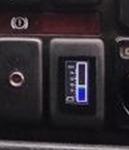
\includegraphics[width=.85\textwidth,height=.60\textheight,keepaspectratio]{figures/ivevo/image16.png}
\caption{Voltmeter}
\end{figure}

\begin{figure}[H]
\centering
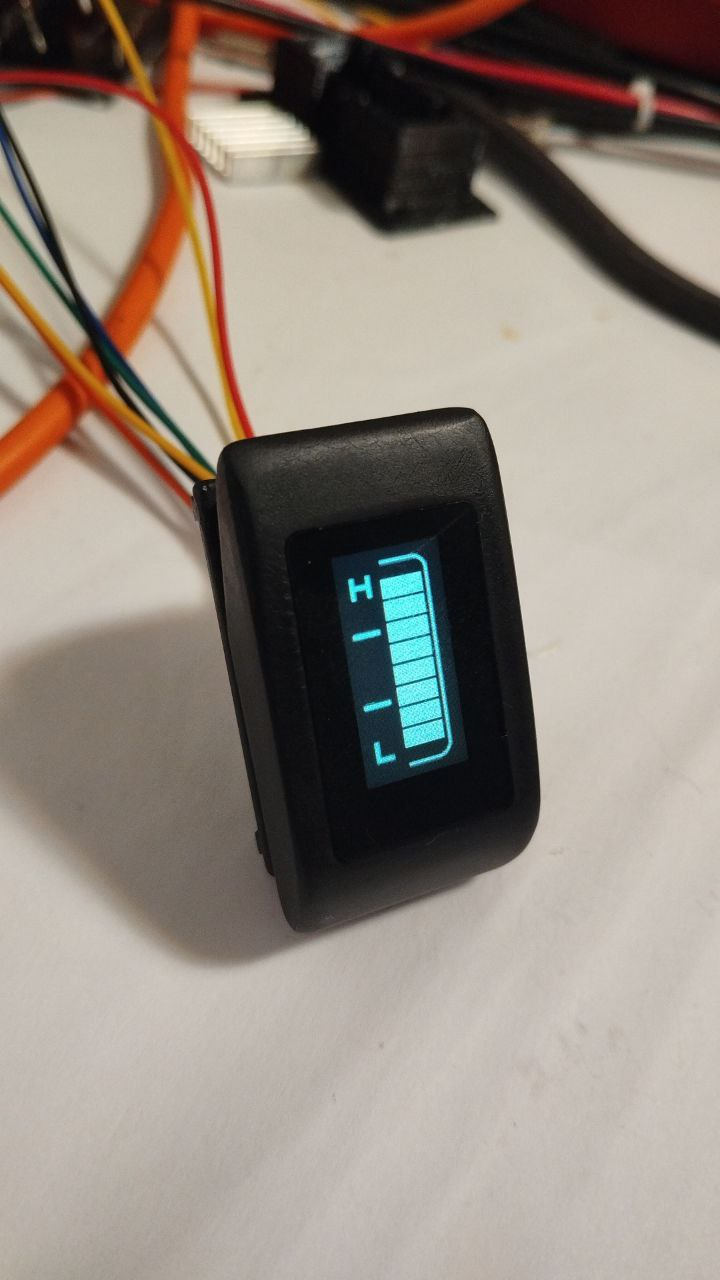
\includegraphics[width=.85\textwidth,height=.60\textheight,keepaspectratio]{figures/ivevo/image15.png}
\caption{Voltmeter}
\end{figure}

\begin{figure}[H]
\centering
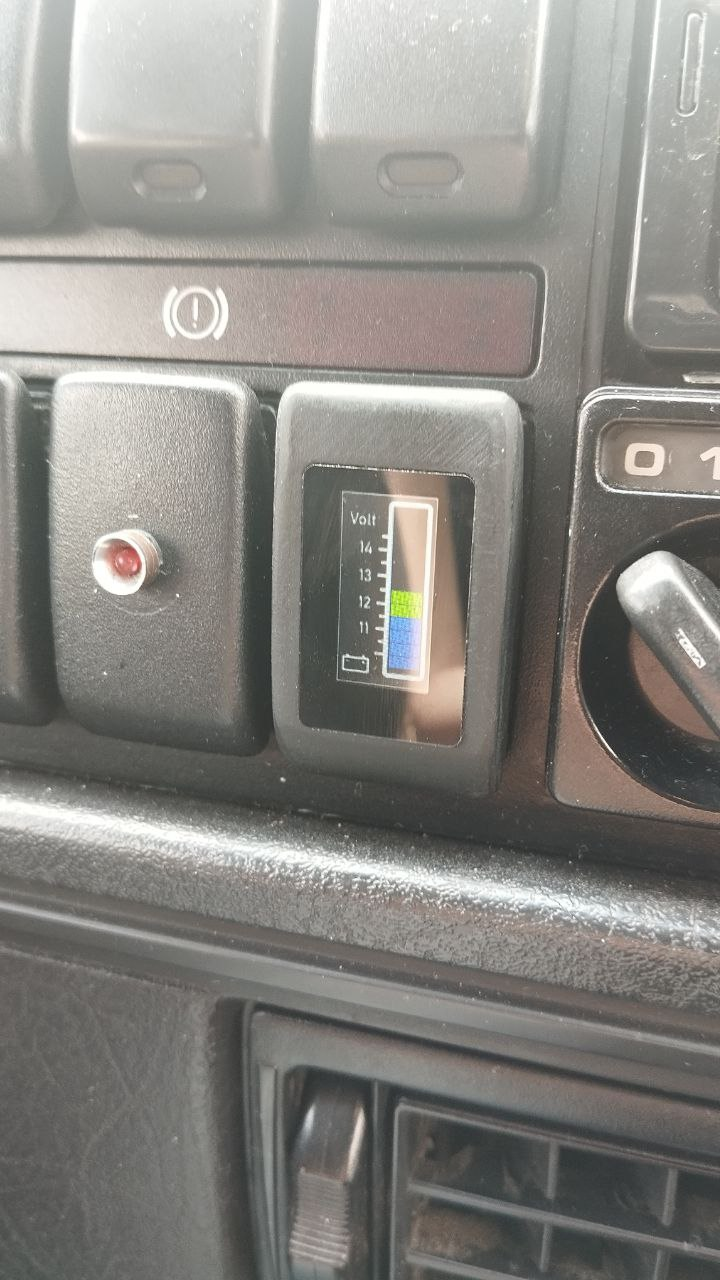
\includegraphics[width=.85\textwidth,height=.60\textheight,keepaspectratio]{figures/ivevo/image2.png}
\caption{Voltmeter}
\end{figure}
\section{Öldruck (Barometer)}
Ein Sensor ist erforderlich; vorgesehen ist VAG 03C906051A. Trotz des internen +5-V-Ausgangs empfiehlt die Vorlage einen externen DC/DC-Wandler für die Sensorversorgung. Den Öldruck-Anschlussplan und eine passende Sensorkalibrierung verwenden.

\begin{figure}[H]
\centering
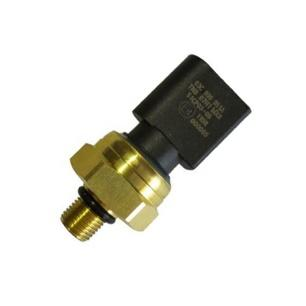
\includegraphics[width=.85\textwidth,height=.60\textheight,keepaspectratio]{figures/ivevo/image21.jpg}
\caption{Öldruck (Barometer)}
\end{figure}
\section{Temperatur (Thermo)}
Entweder einen NTC-Sensor oder einen digitalen DS18B20 mit passendem Sensorskript verwenden. DS18B20-Kabelsonden werden unterstützt. Als NTC wird Ossca 01176 oder ein kompatibler Golf-2-Sensor empfohlen. Am Ossca-Sensor die Sensorpins 1 und 2 verbinden; der NTC-Widerstand liegt an Sensorpin 3. Diese Nummern beziehen sich auf den Sensor, nicht auf die Versorgungspins der Anzeige.

\begin{figure}[H]
\centering
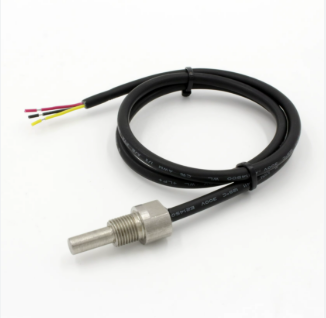
\includegraphics[width=.85\textwidth,height=.60\textheight,keepaspectratio]{figures/ivevo/image14.png}
\caption{Temperatur (Thermo)}
\end{figure}

\begin{figure}[H]
\centering
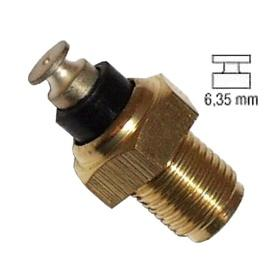
\includegraphics[width=.85\textwidth,height=.60\textheight,keepaspectratio]{figures/ivevo/image19.jpg}
\caption{Temperatur (Thermo)}
\end{figure}
\section{Ganganzeige}
Unterstützt werden R und die Gänge 1–5. Die Anzeige berechnet den Gang aus Geschwindigkeit und Drehzahl des Digifiz Next über Bluetooth LE. Für den Rückwärtsgang ist ein positives Eingangssignal gemäß Anschlussplan erforderlich. Digifiz Next muss Firmware 1.0.14 oder neuer verwenden.

Pin 1 (K30/KL30) für diese Anwendung mit +12 V KL15/Zündungsplus verbinden, Pin 7 mit Fahrzeugmasse. Nach dem Einschalten zeigt ein Strich einen nicht gewählten Gang an; das Gerät sucht nach Digifiz Next. Im QR-Code-Konfigurationsmodus die Anwendung iv\_gear und den Sensor volts1 auswählen, speichern und die Zündung neu einschalten.

Im Digifiz-Next-Webpanel Geschwindigkeit anhand GPS, Drehzahl und Gangtabelle auf das Fahrzeug abstimmen. Die Vorlage empfiehlt 80–100 km/h als Geschwindigkeitsreferenz; nur unter sicheren und zulässigen Bedingungen messen und eine Begleitperson protokollieren lassen. Die genannten Drehzahl-Kalibrierwerte 1500, 3000 und 400 haben keine eindeutige Einheit oder Motorzuordnung. Die motorspezifische Cluster-Anleitung verwenden, keine Werte erraten.

\begin{figure}[H]
\centering
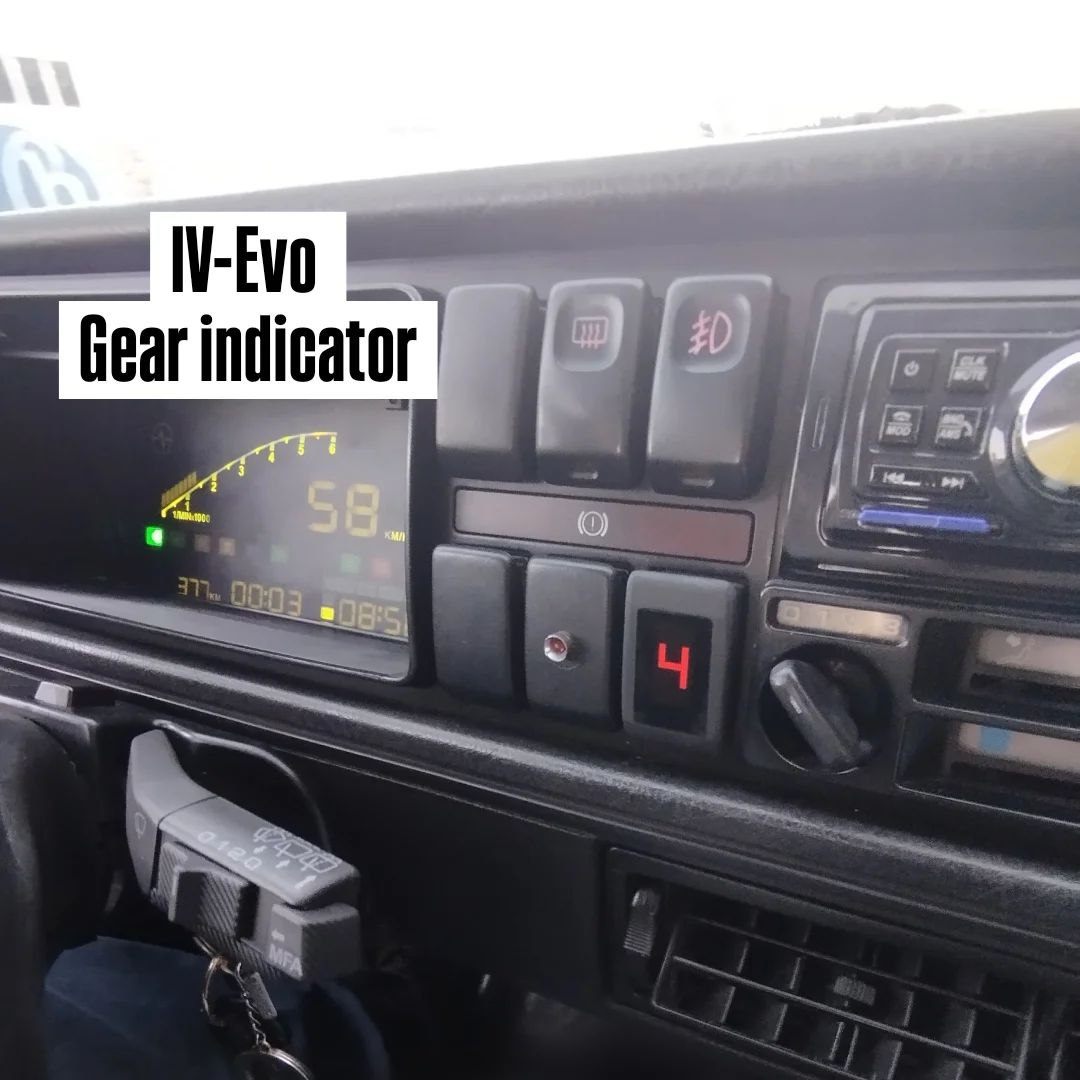
\includegraphics[width=.85\textwidth,height=.60\textheight,keepaspectratio]{figures/ivevo/image18.png}
\caption{Ganganzeige}
\end{figure}

\begin{figure}[H]
\centering
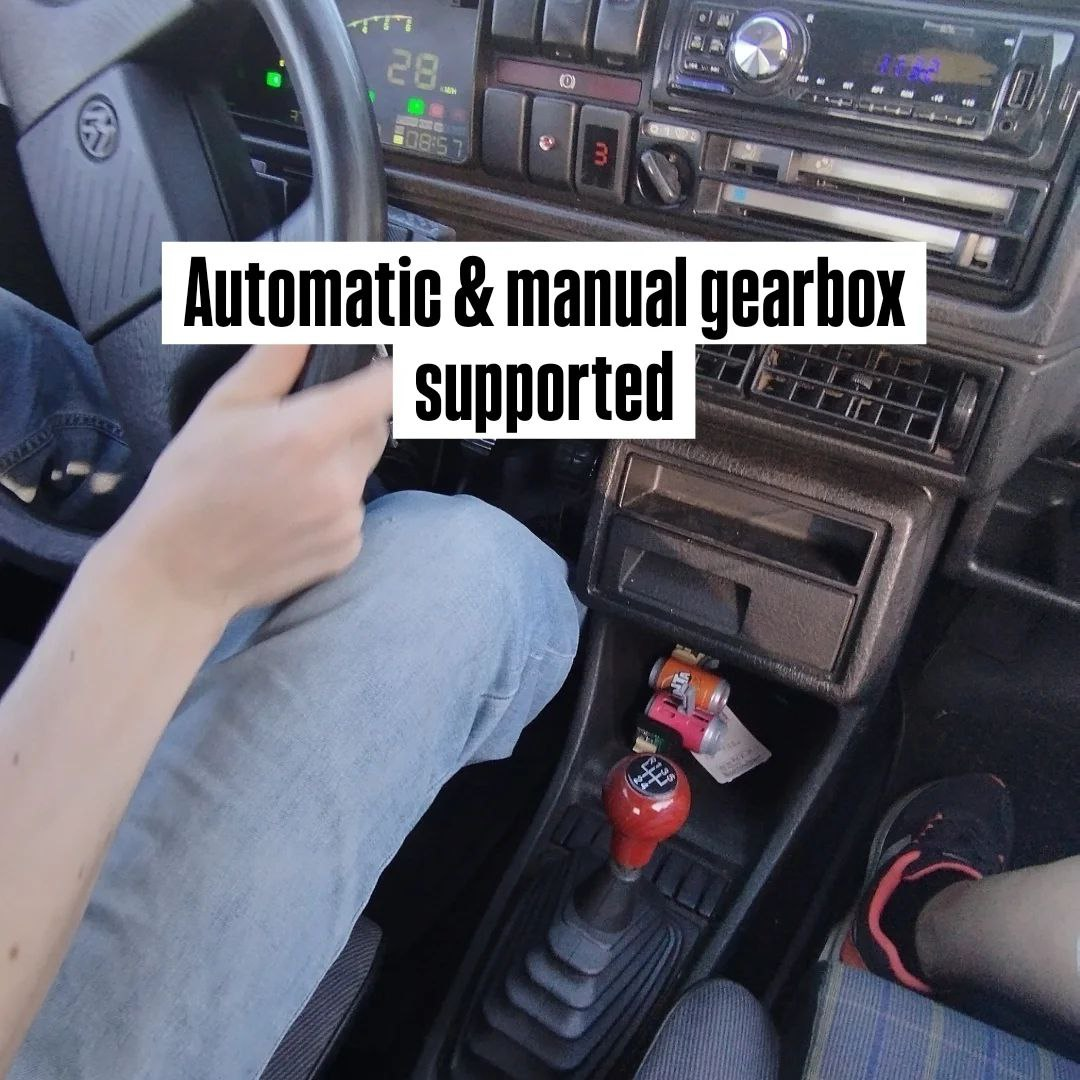
\includegraphics[width=.85\textwidth,height=.60\textheight,keepaspectratio]{figures/ivevo/image10.png}
\caption{Ganganzeige}
\end{figure}
\section{Lambda}
Nicht an die serienmäßige Golf-2-Lambdasonde anschließen. Die Vorlage verlangt eine separate Messsonde; bleibt die Originalsonde erhalten, sind zwei Sonden eingebaut. Eine Sprungsonde liefert etwa 0,1 V (mager) bis 0,9 V (fett) und keine genaue Luft-Kraftstoff-Verhältnis-Messung. Der direkte Anschluss erfordert Kalibrierung.

Eine Breitbandsonde benötigt einen eigenen Controller; IV-Evo kann sie nicht selbst ansteuern. Empfohlen wird Bosch LSU 4.9 mit kompatiblem Controller, etwa SLC Free, DIY-EFI TinyWB, Sigma Lambda Controller Free 2 oder rusEFI wideband. Die Sonde nach Controller-Anleitung anschließen und dessen Analogausgang verwenden. Dieser kann 0–5 V, 0,5–4,5 V oder 0–1 V liefern; Eingangszuordnung und Kalibrierkurve müssen dazu passen.

\begin{figure}[H]
\centering
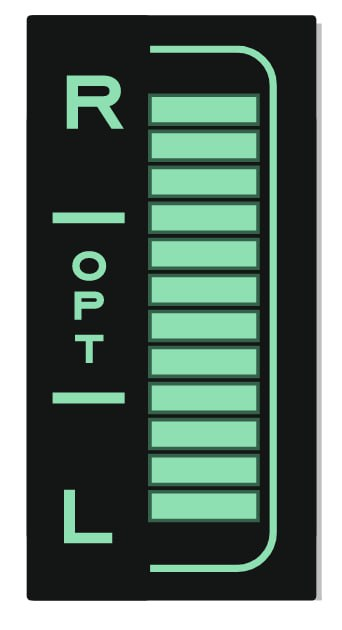
\includegraphics[width=.85\textwidth,height=.60\textheight,keepaspectratio]{figures/ivevo/image7.png}
\caption{Lambda}
\end{figure}
\section{Check Engine}
Bei 12 V an Pin 2 (V2) erscheint „Check Engine“, bei 0 V bleibt die Anzeige leer. Dies ist eine Signalanzeige; Fehlercodeauslesen oder eine OBD-Schnittstelle sind nicht beschrieben.

\begin{figure}[H]
\centering
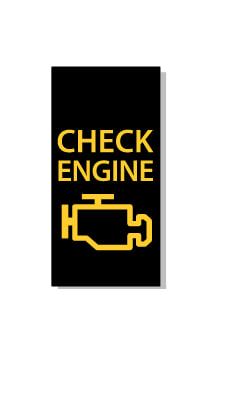
\includegraphics[width=.85\textwidth,height=.60\textheight,keepaspectratio]{figures/ivevo/image4.png}
\caption{Check Engine}
\end{figure}
\section{Ladedruck (Boost)}
Ein Sensor mit drei Pins, +5-V-Versorgung, einer Befestigungsbohrung und 20–250 kPa Messbereich ist angegeben. Die nominale Ausgangsspannung beträgt +1,8 V. Der zugehörige Druck und die vollständige Übertragungsfunktion fehlen. Vor der Kalibrierung den genauen Sensortyp und seine Kennlinie bestätigen; aus einem einzigen Wert keine Steigung ableiten.

\begin{figure}[H]
\centering
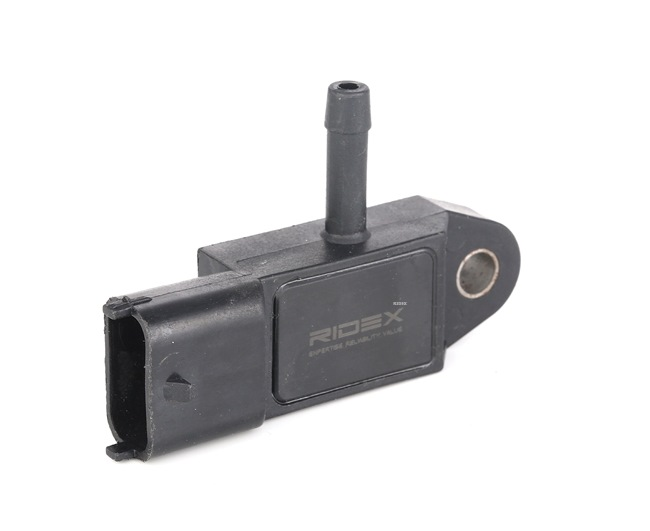
\includegraphics[width=.85\textwidth,height=.60\textheight,keepaspectratio]{figures/ivevo/image9.png}
\caption{Ladedruck (Boost)}
\end{figure}
\section{Uhr}
Die Beispielanwendung nutzt die Systemzeit. Nach einem Neustart bleibt die Uhrzeit nicht erhalten; ohne erneutes Stellen dient die Anzeige als Fahrtzeitzähler.

\begin{figure}[H]
\centering
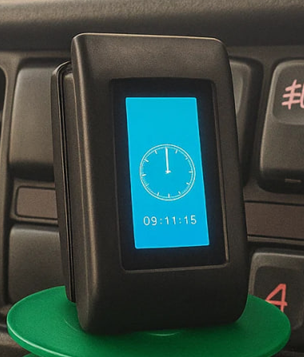
\includegraphics[width=.85\textwidth,height=.60\textheight,keepaspectratio]{figures/ivevo/image12.png}
\caption{Uhr}
\end{figure}
\section{Grenzen der Dokumentation}
Allgemeine Versorgungstoleranzen, Betriebstemperaturen und eine Gehäuse-Schutzart sind nicht angegeben. Nano-Spezifikationen nicht auf IV-Evo übertragen.
